% This is samplepaper.tex, a sample chapter demonstrating the
% LLNCS macro package for Springer Computer Science proceedings;
% Version 2.21 of 2022/01/12
%
\documentclass[runningheads]{llncs}
%
\usepackage[T1]{fontenc}
% T1 fonts will be used to generate the final print and online PDFs,
% so please use T1 fonts in your manuscript whenever possible.
% Other font encondings may result in incorrect characters.
%
\usepackage{graphicx}

% Used for displaying a sample figure. If possible, figure files should
% be included in EPS format.
%
% If you use the hyperref package, please uncomment the following two lines
% to display URLs in blue roman font according to Springer's eBook style:
\usepackage{color}
%\renewcommand\UrlFont{\color{blue}\rmfamily}
%
\begin{document}
%
\title{Contribution Title\thanks{Supported by organization x.}}
%
%\titlerunning{Abbreviated paper title}
% If the paper title is too long for the running head, you can set
% an abbreviated paper title here
%
\author{First Author\inst{1}\orcidID{0000-1111-2222-3333} \and
Second Author\inst{2,3}\orcidID{1111-2222-3333-4444} \and
Third Author\inst{3}\orcidID{2222--3333-4444-5555}}
%
\authorrunning{F. Author et al.}
% First names are abbreviated in the running head.
% If there are more than two authors, 'et al.' is used.
%
\institute{Princeton University, Princeton NJ 08544, USA \and
Springer Heidelberg, Tiergartenstr. 17, 69121 Heidelberg, Germany
\email{lncs@springer.com}\\
\url{http://www.springer.com/gp/computer-science/lncs} \and
ABC Institute, Rupert-Karls-University Heidelberg, Heidelberg, Germany\\
\email{\{abc,lncs\}@uni-heidelberg.de}}
%
\maketitle              % typeset the header of the contribution
%
\begin{abstract}
The abstract should briefly summarize the contents of the paper in
150--250 words.

\keywords{First keyword  \and Second keyword \and Another keyword.}
\end{abstract}
%
%
%
\section{First Section}
\begin{table}
	\caption { Arabic AI Models Studies in Retrieval-Augmented Generation (RAG)  }\label{tab:arabic_rag}
	\centering
	\resizebox{\textwidth}{!}{ 
		\begin{tabular}{|p{3.5cm}|p{1.4cm}|p{3.5cm}|p{4.5cm}|p{3cm}|p{3.5cm}|p{3.5cm}|}
		\hline
		\multicolumn{7}{|c|}{\textbf{Studies on Retrieval-Only Models}} \\
		\hline
			\textbf{Paper} & \textbf{year} &
		    \textbf{Retrieval Component Studied} 	& 
		    \textbf{Arabic Model Name} & \textbf{Datasets Used} & \textbf{Evaluation Metrics} & \textbf{Addressed Challenges}  \\
			\hline
			Semantic Embeddings for Arabic Retrieval
			Augmented Generation (ARAG) \cite{ref_arag2023} & 2023 &\textbf{Retrieval} :Semantic   Embeddings &
			Microsoft(e5s,e5b,e5l)\newline DistillBert(hf1,hf2),\newline Openai  Ada embedding \newline  Cohere Multilingual Embedding \newline Meta SONAR  \newline Google LaBSE\newline mpnet-base-v2   & Arabic Reading Comprehension Dataset (ARCD) & Recall@k.&-Embedding Size Constraints \newline      -Need for Language Specific Evaluation Metrics \\
			\hline
			Evaluation of Semantic Search and its Role in Retrieved for Arabic Language\cite{Mahboub2024} & 2024 &\textbf{Retrieval} :Semantic search in Arabic &Encoder 1: MiniLM \newline
			Encoder 2: CMLM\newline
			Encoder 3: MPNet \newline
		    Encoder 4: DistilBERT\newline
		    Encoder 5 : XLM RoBERTa &FAQs: 816 questions with verifiable answers & NDCG@3 \newline MRR@3 \newline mAP@3 & -Embedding size constraints. \newline -Arabic complexity \\
			\hline
			Arabic RAG Leaderboard: A Comprehensive Framework for Evaluating Arabic Language Retrieval Systems\cite{ref_TARL2025} & 2025&
			\textbf{Retrieval}: Semantic Embedding . \newline 
			\textbf{Reranking}:Refine retrieved documents & Retrieval :GATE-AraBERT-v1 \newline
			Reranking : ARA-Reranker-V1\newline
			 &Retrieval:"Web Search Dataset" \newline Reranking:sourced from TyDi QA and MKQA datasets & NDCG \newline MRR \newline mAP \newline Recall@k &  Arabic’s morphological complexity \newline  Dialect diversity\\
			\hline
	        \multicolumn{7}{|c|}{\textbf{Studies on Both Retrieval and Generation}} \\
	        \hline
	       
	        \textbf{Paper} & \textbf{Year} & \textbf{RAG Component Studied} & \textbf{Arbic  Model Name} & \textbf{Datasets Used} & \textbf{Evaluation Metricsl} & \textbf{Addressed Chalenges} \\
	        \hline
			Exploring Retrieval Augmented Generation in Arabic \cite{ref_elbeltagy2024} & 2024 . &  \textbf{Retrieval}: Semantic Embedding \newline \textbf{Generation} : generate Arabic response  & \textbf{Retrieval}: AraVec , AraBERT ,OpenAI ,Cohere, Microsoft’s E5,  Ollama ,JAIS,BGE \newline \textbf{Generator}:GPT3.5, urbo, Mistral 
			7B, Llama 3, Mixtral, and JAIS.
			  & Ar-EduText dataset, \newline ARCD dataset 
			  &\textbf{Retrival}:Recall@K (k=1,k=3,k=5) \newline \textbf{Generator}: F1 Score Bleu Score Cosine SimilarityR&-Lack of Detailed Metrics \newline -Dialect Diversity \\
			\hline
		Evaluating RAG Pipelines for Arabic Lexical Information Retrieval: A Comparative Study of Embedding and Generation Models\cite{ref_alrasheed2025} & 2025 & \textbf{Retrieval}: Word Embeddings , Sentence Embeddings \newline \textbf{Generator} : generatte Arabic lexical information&\textbf{Retrival}:CAMeLBERT, AraBERT-v2, E5-large Arabic-NLI ,AraELECTRA  \newline \textbf{Generator}: GPT-4o, Gemini-1.5-flash, SILMA-9B-Instruct, Aya8B GPT-3.5, AceGPT13B&Riyadh dictionary (88,000+ words)&\textbf{Retrival} Top-k Recall (k = 1, 3, 5) and MRR \newline \textbf{Generator}:F1-score(F1),
		Accuracy (Acc), and CosineSimilarity(Cos). &-handling of dialectal variations in queries and documents. \newline -Disparity in performance between sentence embeddings and word \\
			\hline
	
		\end{tabular}
	} % End resizebox
\end{table}















%\subsection{A Subsection Sample}


%\subsubsection{Sample Heading} Only two levels of

%\paragraph{Sample Heading (Fourth Level)}







%\begin{figure}
%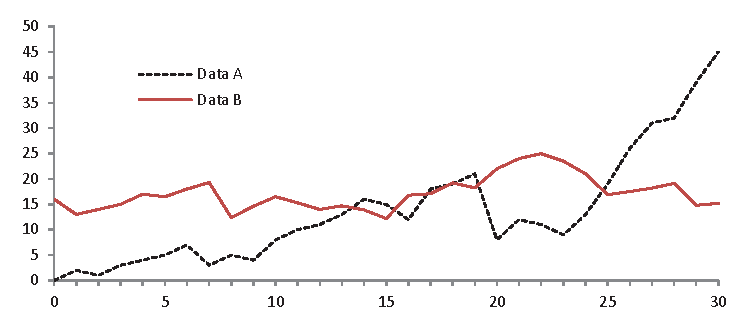
\includegraphics[width=\textwidth]{fig1.eps}
%\caption{A figure caption is always placed below the illustration.
%Please note that short captions are centered, while long ones are
%justified by the macro package automatically.} \label{fig1}
%\end{figure}%



% the environments 'definition', 'lemma', 'proposition', 'corollary',
% 'remark', and 'example' are defined in the LLNCS documentclass as well.
%

%For citations of references, we prefer the use of square brackets
%and consecutive numbers. Citations using labels or the author/year
%convention are also acceptable. The following bibliography provides
%a sample reference list with entries for journal
%articles~\cite{ref_article1}, an LNCS chapter~\cite{ref_lncs1}, a
%book~\cite{ref_book1}, proceedings without editors~\cite{ref_proc1},
%and a homepage~\cite{ref_url1}. Multiple citations are grouped
%\cite{ref_article1,ref_lncs1,ref_book1},
%\cite{ref_article1,ref_book1,ref_proc1,ref_url1}.

%\subsubsection{Acknowledgements} Please place your acknowledgments at
%the end of the paper, preceded by an unnumbered run-in heading (i.e.
%3rd-level heading).

%
% ---- Bibliography ----
%
% BibTeX users should specify bibliography style 'splncs04'.
% References will then be sorted and formatted in the correct style.
%
% \bibliographystyle{splncs04}
% \bibliography{mybibliography}
%
\newpage
\begin{thebibliography}{8}
\bibitem{ref_arag2023}
Abdelazim, H., Mohamed, A., Tharwat, M.: Semantic Embeddings for Arabic Retrieval Augmented Generation (ARAG). International Journal of Advanced Computer Science and Applications \textbf{14}(11), xx--yy (2023)


\bibitem{Mahboub2024}
Mahboub, A., Za’ter, M. E., Al-Rfooh, B., Estaitia, Y., Jaljuli, A., Hakouz, A.:  
Evaluation of Semantic Search and its Role in Retrieved-Augmented-Generation (RAG) for Arabic Language.  
In: arXiv preprint, arXiv:2403.18350v2, May 2024. Available at: \url{https://arxiv.org/abs/2403.18350}

\bibitem{ref_TARL2025}
Rashad, M.A., Shahid, H.: The Arabic RAG Leaderboard. \textit{Navid-AI} (2025). Available online at: \url{https://huggingface.co/spaces/Navid-AI/The-Arabic-Rag-Leaderboard}.


\bibitem{ref_elbeltagy2024}
El-Beltagy, S.R., Abdallah, M.A.: Exploring Retrieval Augmented Generation in Arabic. Procedia Computer Science, \textbf{00}, 000--000 (2024). Available online at: \url{www.sciencedirect.com}.

\bibitem{ref_alrasheed2025}
Al-Rasheed, R., Al Muaddi, A., Aljasim, H., Al-Matham, R., Alhoshan, M., Al Wazrah, A., AlOsaimy, A.:  
Evaluating RAG Pipelines for Arabic Lexical Information Retrieval: A Comparative Study of Embedding and Generation Models.  
In: El-Haj, M. (ed.), Proc. 1st Workshop on NLP for Languages Using Arabic Script, pp. 155--164.  
Association for Computational Linguistics, Abu Dhabi, UAE (2025).  
Available: \url{https://aclanthology.org/2025.abjadnlp-1.16/}  




\bibitem{ref_proc1}
Author, A.-B.: Contribution title. In: 9th International Proceedings
on Proceedings, pp. 1--2. Publisher, Location (2010)

\bibitem{ref_url1}
LNCS Homepage, \url{http://www.springer.com/lncs}. Last accessed 4
Oct 2017
\end{thebibliography}
\end{document}
